% ！！重点写一些创新的东西，不是流水账式的。

\section{Formalization of CIRCT Dialects Semantics}\label{sec:semantics-formalization}

In this section, we explore the semantics of CIRCT, consisting of MLIR static semantics, CIRCT static semantics, and dynamic semantics for HW, COMB, SEQ, and SV. \red{For each semantics, we will present a language overview, define the execution state, elucidate semantic phases, and provide sample semantic rules to illustrate the construction of semantics, as necessary.}

\subsection{MLIR Static Semantics}\label{sec:mlir-static-semantics}

MLIR aims to represent a wide range of concepts across different abstraction levels through a unified language utilizing an extension mechanism called ``dialects''. Within the context of the CIRCT project, a set of dialects is developed to represent circuits at various abstraction levels. Consequently, our approach involves first formalizing the semantics of MLIR before delving into the semantics of CIRCT, which is designed to streamline the formalization of dialect semantics.

To meet this design objective, we must maximize the incorporation of the MLIR concept within the $\mathbb{K}$ definition while avoiding the introduction of dialect-specific elements. This results in three key components: (1) a generic MLIR syntax for parsing and describing dialect semantics, (2) a program configuration for housing the normalized program, and  (3) semantic phases for normalizing the original program.

\smallskip
\textbf{Generic MLIR Syntax}. Generic MLIR is a representation format that MLIR compiler can transform any customized dialect MLIR into. Thus we can parse and describe arbitrary MLIR program with any dialects after formalizing the generic MLIR in $\mathbb{K}$. According to the reference~\red{https://mlir.llvm.org/docs/LangRef/}, we define the syntax of generic MLIR in $\mathbb{K}$, and use the $\mathbb{K}$ generated parser to parse the real program to avoid the ambiguity in documentation. \red{Indeed, we find some documents errors when we define the syntax which will be discussed in Section~\ref{sec:validation}.} 

\begin{figure}
\[\begin{aligned}
&\text{TopLevel}&
\syn{toplevel} \Coloneqq &\ \scmd{(} \syn{operation} \scmd{$\mid$} \syn{type-alias-def} \scmd{$\mid$} \syn{attr-alias-def} \scmd{)*}
\\
&\text{Operation}&
\syn{operation} \Coloneqq &\ \scmd{(} \syn{op-results}\ \tok{=} \scmd{)?}\ \syn{str}\ \tok{(} \scmd{(}\syn{value-uses}\scmd{)?} \tok{)}\ \scmd{(}\tok{[} \syn{successors} \tok{]}\scmd{)?}\ %\scmd{(}\tok{<}\ \syn{dict-attr} \ \tok{>}\scmd{)?}\ 
\scmd{(}\tok{(} \syn{regions} \tok{)}\scmd{)?}
\\ 
& &
&\ \scmd{(} \tok{\{} \scmd{(}\syn{dict-attr}\scmd{)?} \tok{\}}\scmd{)?}\ \tok{:}\ \syn{fun-type}\ \scmd{(}  \syn{loc-attr} \scmd{)?}
\\
& &
\syn{op-results} \Coloneqq &\ \syn{op-result}\ \scmd{(} \tok{,}\ \syn{op-result} \scmd{)*} \hspace{30pt} \syn{op-result} \Coloneqq \ \tok{\%}\syn{id}\ \scmd{(} \tok{:}\ \syn{int} \scmd{)?}
\\
& &
\syn{value-uses} \Coloneqq &\ \syn{value-use}\ \scmd{(} \tok{,}\ \syn{value-use} \scmd{)*} \hspace{22pt} \syn{value-use} \Coloneqq \ \tok{\%}\syn{id}\ \scmd{(} \tok{\#}\ \syn{int} \scmd{)?}
\\
& &
\syn{successors} \Coloneqq &\ \syn{successor}\ \scmd{(} \tok{,}\ \syn{successor} \scmd{)*} \hspace{26pt} \syn{successor} \Coloneqq \ \tok{\^}\syn{id}\ \scmd{(}\tok{:}\ \tok{(} \syn{block-args} \tok{)} \scmd{)?}
\\
&\text{Region}& \syn{regions} \Coloneqq &\ \syn{region}\ \scmd{(} \tok{,}\ \syn{region} \scmd{)*} \hspace{61pt} \syn{region} \Coloneqq \ \tok{\{} \syn{operation}^\scmd{+}\ \syn{block}\scmd{*} \tok{\}}
\\
&\text{Block}& \syn{block} \Coloneqq &\ \syn{block-label}\ \syn{operation}^\scmd{+} \hspace{21pt} \syn{block-label} \Coloneqq \ \tok{\^}\syn{id} \ \scmd{(} \tok{(} \syn{block-args} \tok{)} \scmd{)?}\ \tok{:}
\\
& &
\syn{block-args} \Coloneqq &\ \scmd{(} \tok{\%}\syn{id}\ \tok{:}\ \syn{type} \scmd{(} \tok{,}\ \tok{\%}\syn{id}\ \tok{:}\ \syn{type} \scmd{)*} \scmd{)?}
\\
&\text{Type}&
\syn{type-alias-def} \Coloneqq &\ \syn{type-alias} \ \tok{=} \ \syn{type} \hspace{46pt} \syn{type-alias} \Coloneqq \ \tok{!}\syn{bare-id}
\\
& & \syn{func-type} \Coloneqq  &\ \scmd{(} \syn{type} \scmd{$\mid$} \tok{(} \syn{types} \tok{)} \scmd{)} \tok{->} \scmd{(} \syn{type} \scmd{$\mid$} \tok{(} \syn{types} \tok{)} \scmd{)} \hspace{17pt} \syn{types} \Coloneqq \ \syn{type}\ \scmd{(} \tok{,}\ \syn{type} \scmd{)*}
\\
& &
\syn{type} \Coloneqq &\ \syn{type-alias} \scmd{$\mid$} \syn{dialect-type} \scmd{$\mid$} \syn{builtin-type}
\\
&\text{Attribute}&
\syn{attr-alias-def} \Coloneqq &\ \syn{attr-alias}\ \tok{=}\ \syn{attr-value} \hspace{30pt} \syn{attr-alias} \Coloneqq \ \tok{\#}\syn{bare-id}
\\
& &
\syn{dict-attr} \Coloneqq &\ \syn{attr-entry} \ \scmd{(} \tok{,}\ \syn{attr-entry} \scmd{)*} \hspace{19pt} \syn{attr-entry} \Coloneqq \ \scmd{(} \syn{id} \scmd{$\mid$} \syn{str}  \scmd{)} \ \tok{=} \ \syn{attr-value} 
\\
& & \syn{loc-attr} \Coloneqq &\ \tok{loc} \tok{(} \syn{location} \tok{)}
\\
& &
\syn{attr-value} \Coloneqq &\ \syn{attr-alias} \scmd{$\mid$} \syn{dialect-attr} \scmd{$\mid$} \syn{builtin-attr} \hspace{7.5em} 
\\
\end{aligned}\]
\caption{Syntax for generic MLIR. Note that this figure omits some syntax definitions (e.g., \syn{builtin-attr} --- the builtin attributes of MLIR) due to the limited space. Indeed, K-CIRCT consists of all the syntax definitions.}
\label{fig:mlir-syntax}
\end{figure}

Fig.~\ref{fig:mlir-syntax} shows (a fragment of) the syntax for the generic MLIR formalized in K-CIRCT. The variables \syn{id} and \syn{bare-id} represent two kinds of tokens for MLIR identifiers. The variable \syn{id} can start with numbers to construct identifiers for values (e.g., $\%1$, $\%2$, $\%3$, etc.) and blocks (e.g., $\textasciicircum\$$, $\textasciicircum\text{-}$, $\textasciicircum1$, etc.). In contrast, the variable \syn{bared-id} can only start with letters or \_ to present type aliases (e.g., $!\_$, $!A$, $!b$, etc.) and attribute aliases (e.g., $\#x$, $\#y$, $\#z$, etc.). Moreover, the operations leverage strings \syn{str} to identify themselves, such as $``hw.module"$, $``comb.add"$, $``sv.always"$, etc.


Each MLIR source file contains a list of operations \syn{operation}, type alias definitions \syn{type-alias-def}, and attribute alias definitions \syn{attr-alias-def}.  Fig.~\ref{fig:circt-example} shows a small example of MLIR/CIRCT syntax, whose meaning we explore with more detail in Section~\ref{sec:core-dialect-semantics}.

\begin{figure}
\centering
\begin{lstlisting}
    hello world
\end{lstlisting}
\caption{An example use of CIRCT's core dialects. Here, \red{blabla}. \red{It should be an example that includes all the important features under explanation, such as normalize, symbol table, preprocess, stimulate, hw.module, comb.add, seq.???, sv.???}}
\label{fig:circt-example}
\end{figure}

Operations \syn{operation} present a unified behavior structure for all the possible representations with different abstraction levels. Given any string \syn{str} to identify the operation, it can compute with a list of values \syn{value-uses} and possibly assign the result to another list of values \syn{op-results}. The function types \syn{func-type} are used to indicate the types of the results and operands. The operations can be expressions and instructions with merely a dictionary of attributes \syn{dict-attr} to declare some attribute to some specific parameter, and a location attribute \syn{loc-attr} to give its location in the source code for traceability. The operations can also be functions and modules with zero or more successors \syn{successor} and a list of regions \syn{region} as the body of the functions or modules.

Regions \syn{region} and Blocks \syn{block} provide a recursive and nesting structure for the operation body. Specifically, the regions contain a list of blocks; the blocks contain a list of operations; the operations contain further regions. The semantics of the regions are determined by the attached operations and their attributes, while the blocks form a Control Flow Graph (CFG). Each block ends with a terminator operation, that may have successor blocks in the same region or return it to the enclosing region. Terminators in MLIR pass values into block arguments \syn{block-args} defined by the successor block to provide an alternative for LLVM $\phi$ node.

Types \syn{type} and Attributes \syn{attr-value} can be aliases defined in the MLIR source file, dialect attributes predefined in the dialect implementations or built-in attributes predefined in the MLIR implementation. Types encode the data knowledge, while attributes represent the data.

\begin{figure}[ht]
\centering
\begin{small}
\[
\left\langle
\begin{aligned}
\langle \syn{toplevel} \rangle_{prog} \hspace{3pt}
\langle \syn{operation}\scmd{*}\rangle_{std-op} \hspace{3pt}
\langle \syn{type-alias} \mapsto \syn{type} \rangle_{types}
\\
\langle \syn{attr-alias} \mapsto \syn{attr-value} \rangle_{attrs} \hspace{3pt}
\langle \syn{str} \mapsto \syn{operation} \rangle_{sym-tab} 
\end{aligned}
\right\rangle_{mlir}
\]
\end{small}
\caption{The program configuration for MLIR.}
\label{fig:mlir-conf}
\end{figure}

\smallskip
\textbf{Program Configuration}. After defining the syntax of MLIR, the MLIR semantics require a program configuration to specify the runtime state. Each cell is separated by the angle brackets with its name on the bottom right. The \textit{mlir} cell contains the cells related to MLIR semantics. The \textit{prog} cell begins with the MLIR source file in the type of \syn{toplevel}, while the other cells are initialized by an empty list or map. Since the \textit{std-op}, \textit{types}, \textit{attrs} and \textit{sym-tab} cells contain the result of MLIR static semantics, we describe these cells in the below semantic phases.

\smallskip
\textbf{Semantic Phases}. The MLIR static semantics aim to streamline the semantics development of dialects. Thus, we present the following phases to eliminate focus on the syntax differences and mechanisms for accessing the operations at the dialect semantics level.

\smallskip
\textit{Normalize Operations}. As we can see in the MLIR syntax (Fig.~\ref{fig:mlir-syntax}), many possible structure exists in \syn{toplevel} and \syn{operation}. This leads to the development complexity of the semantics since we need to cover all the syntax possibilities. Thus we introduce the operation normalization phase for MLIR static semantics to reduce this complexity for the dialect semantics. This phase stores the type alias definitions \syn{type-alias-def} and attribute alias definitions \syn{attr-alias-def} into the \textit{type} and \textit{attrs} cells, respectively, providing a standard and more accessible format for them. Additionally, this phase fills each absent syntactic unit (e.g., \scmd{(}\syn{op-results}\tok{=}\scmd{)?}) with a semantic empty unit (e.g., \syn{.op-results =}\footnote{Syntactic units with a ``.'' means a semantic empty unit for its corresponding syntactic unit.}), and stores them into the \textit{std-op} cell. \red{For example} This way, we eliminate the possibility of \syn{toplevel} and \syn{operation} for dialect semantics, improving their conciseness and development efficiency. 

\smallskip
\textit{Construct Symbol Table}. Requirements for accessing an operation also lead to development complexity, while the nesting structure of MLIR further improves this complexity. This necessitates a symbol table --- a flat and accessible structure --- to facilitate the operation access. We construct the symbol table at the MLIR level and store them in the \textit{sym-tab} cell. The cell contains a map from the symbol name to the normalized operation. During the construction, we delve into every nesting structure of the source file, therefore flattening the operations.

\red{In summary?} With the above components, we define dialect-agnostic and usable semantics at the MLIR level, which can be used for all the other dialects, including the \textit{builtin} dialect.

\subsection{CIRCT Static Semantics}\label{sec:circt-static-semantics}

\red{language overview}

\smallskip
\textbf{Program Configuration}. After defining the syntax of MLIR, the MLIR semantics require a program configuration to specify the runtime state. Each cell is separated by the angle brackets with its name on the bottom right. The \textit{mlir} cell contains the cells related to MLIR semantics. The \textit{prog} cell begins with the MLIR source file in the type of \syn{toplevel}, while the other cells are initialized by an empty list or map. Since the \textit{std-op}, \textit{types}, \textit{attrs} and \textit{sym-tab} cells contain the result of MLIR static semantics, we describe these cells in the below semantic phases.

\smallskip
\textbf{Semantic Phases}. The MLIR static semantics aim to streamline the semantics development of dialects. Thus, we present the following phases to eliminate focus on the syntax differences and mechanisms for accessing the operations at the dialect semantics level.

\smallskip
\textit{Normalize Operations}. As we can see in the MLIR syntax (Fig.~\ref{fig:mlir-syntax}), many possible structure exists in \syn{toplevel} and \syn{operation}. This leads to the development complexity of the semantics since we need to cover all the syntax possibilities. Thus we introduce the operation normalization phase for MLIR static semantics to reduce this complexity for the dialect semantics. This phase stores the type alias definitions \syn{type-alias-def} and attribute alias definitions \syn{attr-alias-def} into the \textit{type} and \textit{attrs} cells, respectively, providing a standard and more accessible format for them. Additionally, this phase fills each absent syntactic unit (e.g., \scmd{(}\syn{op-results}\tok{=}\scmd{)?}) with a semantic empty unit (e.g., \syn{.op-results =}\footnote{Syntactic units with a ``.'' means a semantic empty unit for its corresponding syntactic unit.}), and stores them into the \textit{std-op} cell. \red{For example} This way, we eliminate the possibility of \syn{toplevel} and \syn{operation} for dialect semantics, improving their conciseness and development efficiency.

\smallskip
\textit{Construct Symbol Table}. Requirements for accessing an operation also lead to development complexity, while the nesting structure of MLIR further improves this complexity. This necessitates a symbol table --- a flat and accessible structure --- to facilitate the operation access. We construct the symbol table at the MLIR level and store them in the \textit{sym-tab} cell. The cell contains a map from the symbol name to the normalized operation. During the construction, we delve into every nesting structure of the source file, therefore flattening the operations.

\red{In summary?} With the above components, we define dialect-agnostic and usable semantics at the MLIR level, which can be used for all the other dialects, including the \textit{builtin} dialect.

\subsection{CIRCT Static Semantics}\label{sec:circt-static-semantics}

\red{language overview}

We can simply devide our our semantics of Circt into two parts: static semantics and dynamical semantics, for parsing modules and simluation respectively. In the static semantics, the symbol table of modules is established, the initial block and always block are registered. In the dynmaic semantics, with given testbench signals, the logic of specified top module are executed clock by clock.

Our semantics are based on the states. States represents the status and inside logic of modules. Semantics is embodied by the change of states. The semantics unit in Circt is operation. For each operation defined in the specification of Circt, we define how should corresponding states change by rewrite rules.

We use configurations to express the runtime states of programs. A configuration is a collection of cells. Cells store states of programs and can be nested. Besides, cells can be added or removed dynamically to work with modular hardware design.

\begin{figure}
\centering
\begin{gather*}
\Biggl\langle
    \left\langle K\right\rangle_{k}
    \left\langle \cdots \right\rangle_{mlir}
    \left\langle \cdots \right\rangle_{circt}
\Biggr\rangle_{Top}\\
\Biggl\langle
\begin{aligned}
    \left\langle Map \right\rangle_{attr-alias}
    \left\langle Map \right\rangle_{type-alias}
    \left\langle Map \right\rangle_{symbol-table}
    \left\langle Map \right\rangle_{inital}
    \left\langle Map \right\rangle_{always}
\end{aligned}
\Biggr\rangle_{mlir}\\
\Biggl\langle
    \left\langle Map\right\rangle_{macros}
    \left\langle \langle\cdots\rangle^*_{frame} \right\rangle_{frames}
\Biggr\rangle_{circt}\\
\Biggl\langle
    \left\langle K \right\rangle_{exec}
    \left\langle Map\right\rangle_{locals}
    \left\langle Map\right\rangle_{output}
\Biggr\rangle_{frame}\\
\Biggl\langle
    \left\langle K \right\rangle_{module}
    \left\langle Map\right\rangle_{signal}
\Biggr\rangle_{simulation}
\end{gather*}
\caption{Configurations of our semantics. The first cell show the structure of the whole configuration. The second and third cells are details of omited parts (expressed by $\cdots$) in the $mlir$ cell and the $circt$ cell. The $*$ symbol of the $frame$ cell is to denote the outer $frames$ cell consists of zero or many $frame$ cells. The fourth cell is the detailed struture of the $frame$ cell.}
\end{figure}

The configuration of Circt consists of four part:
\begin{itemize}
    \item The $\langle K\rangle_k$ cell is a built-in cell in the $\mathbb{K}$ framework which contains a sequence of captured patterns to compute. A pattern in the k cell can be of any defined sort. There is a special sort in $\mathbb{K}$ framework called KItem. Every sort is a sub-sort of KItem. Hence in other words, the k cell consists of KItems.
    
    \item The $\langle \cdots\rangle_{mlir}$ cell is stores meta data at the MLIR level, like symbols of hardware modules, aliases of attributes, the \verb|always| block and \verb|initial| block bound with modules. These information is stored as sub-cells. This part of configuration is established in the parsing phase and provides supports for the simulation phase. The state transition of this cell express the static semantics of CIRCT.
    
    \item The $\langle \cdots\rangle_{circt}$ cell stores states about simulation, including macros and module frames. A module frame is a context corresponding to a module instance in the simulation phase, expressed as a nested cell. Frames is dynamically added or removed with the logically entering and going out of module instances. States in a frame includes the current processed operation, local variables, the output of the current module, and so on, expressed as sub-cells.

    \item The $\langle \cdots\rangle_{simulation}$ cell stores the input signals and the name of the specified module in the simulation phase.
\end{itemize}
To be compatited with $\mathbb{K}$ framework, we can use XML format to express the configuration.
\begin{lstlisting}
<Top>
    <k> .K </k>
    <mlir>
        <mlir-program> $PGM:TopLevel </mlir-program>
        <attr-alias> .Map </attr-alias>
        <type-alias> .Map </type-alias> 
        <symbol-table> .Map </symbol-table>
        <initial> .Map </initial>
        <always> .Map </always>
    </mlir>
    <circt>
        <frames>
            <frame*>
                <exec> .K </exec>
                <locals> .Map </locals>
                <output> .Map </output>
                <local-last>.Map</local-last>
            </frame*>
        </frames>
        <macros>.Map</macros>
    </circt>
    <simluation>
        <module> $MOUDLE:Id </module>
        <signal> $SIGNAL:Map </signal>
    </simulation>
</Top>
\end{lstlisting}

The names of configuration cells are distinct. This gives us convenience to specify a related cell in rewrite rules without its parent cells. For example, the following two rules are identical semantically.
\begin{lstlisting}
rule <k> ... </k>
    <mlir>
        <mlir-program> Op:Operation Ops:OperationList => Ops </mlir-program>
    </mlir>

rule <k> ... </k>
    <mlir-program> Op:Operation Ops:OperationList => Ops </mlir-program>
\end{lstlisting}

\smallskip
\textbf{Program Configuration}.
The configuration of Circt consists of three part, the execution control, the MLIR related part and the circt dialect related part, respectively.

The execution control is implemented with a single \verb|k| cell. We have defined serveral execution phases, including preprocessing, extracting symbols of operations, extracting macros, simulating module with activities, etc.

The MLIR related part includes several meta information of Circt on the MLIR language level, such as the symbol table of operations for reference, the aliases of types and attributes.

The part for circt dialects simulate a runtime model of a circuit module for each time clock, including local variables (old values of the last clock and new values in the current clock), the computating operation sequence (expressing the logic structure of the module), the output of the current module which can be fetched by other modules, and other event registrations (like clock edges) with corresponding event handlers (mainly used for the \verb|always| statements).

\smallskip
\textbf{Semantic Phases}.
The semantic execution base on the time clock. Since 

\smallskip
\textit{Preprocess}.
Before the preprocess phase, we extract infomation about MLIR. For circuit modules (defined by \verb|hw.module| operation), the simulation engine parse them and find their symbol names and construct a symbol table for module reference. Besides, for convenience, the engine will transform every operation into a generic format. For attribute aliases, such as the following location alias:
\begin{lstlisting}[basicstyle=\scriptsize\ttfamily]
#loc = loc("test/main.mlir":2:18)
\end{lstlisting}
This line gives the source code location: the 18th character of the 2nd line in the \verb|test/main.mlir| file, an alias as \verb|#loc|, which can be referenced by other operations as attributes. This is useful for error information reporting. A map is prepared for the attribute alias relation, as a part of the MLIR meta information.

After the MLIR information is processed, there are still a lot meta data inside modules like macros. We analyze these data in the preprocess phase. For instance, the \verb|sv.ifdef| operation defines different behaviors according to whether a macro is defined.
\begin{lstlisting}[basicstyle=\scriptsize\ttfamily]
rule <k> (B:Bool => .K) ~> 
        (
            "sv.ifdef" ( .ValueIdList ) ( R1:Region, R2:Region ) { _:Map } : _:FuncType
            => #if B #then R1 #else R2 #fi
        )
        ...
    </k>
\end{lstlisting}

The preprocessing is recursive, for nested operations, the engine process them like generic program blocks.

After the preprocessing, the runtime model is ready to start the semantic simulation of a specified module.

\smallskip
\textit{Stimulate HW Module}.

Circuit modules in circt are defined with the \verb|hw.module| operation. As we specified, the semantic simulation engine find the coresponding module in the MLIR symbol table by module name, and then initialize a new module frame to simulate a clock activitiy for it. If there is no module found for the specified module name, the engine will throw an error. The input of module is also required.

For example, here is a simple adder module in Circt, which makes an addtion for two 8-bit integers and output an 8-bit ingeger.

\begin{lstlisting}[basicstyle=\scriptsize\ttfamily]
"hw.module"() ({
    ^bb0(%arg0: i1, %arg1: i1, %arg2: i8, %arg3: i8):
        %0 = "comb.add"(%arg2, %arg3) {sv.namehint = "_io_out_T_1"} : (i8, i8) -> i8
        "hw.output"(%0) : (i8) -> ()
}) {
    argLocs = [#loc, #loc1, #loc2, #loc2], 
    argNames = ["clock", "reset", "io_a", "io_b"], 
    comment = "", 
    function_type = (i1, i1, i8, i8) -> i8, 
    parameters = [], 
    resultLocs = [#loc2], 
    resultNames = ["io_out"], 
    sym_name = "Adder"
} : () -> ()
\end{lstlisting}

When the engine starts to simulate the module \verb|Adder|, the input values, two integers are pushed into the module frame as local variables. Then the operation blocks are placed into the execution candicate cell. Usually there are only one operation block in a \verb|hw.module|, which includes several operations, as the main logic of the module. For each operation block, we simulate the operations insied and construct the logic relations.

For \verb|Adder|, the engine will first perform \verb|comb.add| operation for \verb|%arg2| and \verb|%arg3|, that is, make an addition on 8-bit integers, and save the result value to a local variable \verb|%0|. Since the module is simple, the next and also the final operation is to set the local variable \verb|%0| as the output of this module via \verb|hw.output| operation.

\red{discussion and conclusion}

\subsection{Core Dialect Semantics}\label{sec:core-dialect-semantics}

\red{introduction of HW, COMB, SEQ, SV} \red{meaning to CIRCT}

The core content of Circt consists of four dialect: HW, COMB, SEQ, and SV.
\begin{itemize}
    \item The HW dialect is intended to be a generic representation of hardware outside of a particular use-case. It defines some basic concepts in Circt: Hardware structure, Data type, Attrubute, and other miscellaneous operations.

    % Structure
    Circt orginizes hardware components into reusable modules. Each module consists of input, output and inside logic. With HW dialect, we can define a module, instantiate a module, or declare a external module, which makes hardware design more convenitent. Modules interconnect with others through wires. Some hardware logic may have trigger conditions and HW dialect also provides related operations to realize them.
    
    % Data type
    Raw hardware design is established with only bit logic and clock. But nowadays hardwares usually bear more functionalities to pursue better performance, which makes the hardware design more and more complex. It will take more effort to implement the functionalities those can only be implemented by softwares before with the low abstract level of traditional hardware design.
    HW dialects allow users to define composite data structure like Array, Enum, Struct and Union, and provides encapsluted data operations, which hoists the abstract level of hardware design and makes hardware programming more modern. As a kind of intermediate representation of hardware design, Circt benefits a lot from these operations since they have shorten the distance between code and bit logic.
    
    % Attribute
    Attributes are broadly used in Circt. As a fundamental concept in MLIR, attributes allow attach additional information to be attached to operations, types, and other entities within an MLIR program. Attributes makes MLIR expressive and Circt also benefits from them. HW Dialects provide several attribute definition that can be used in Circt to express kinds of attribute value like array, reference, parameter, and  field of composite data type.

    % others
    Besides, HW dialects includes operations to finish some miscellaneous functionalities. For example, bits casting, constant declaration and the data comparsion of Enum type. These functionalities are necessary in Circt but complicated to implement by users.

    \item The COMB dialect is intended to be a generic representation of combinational logic outside of a particular use-case. Operations in the COMB dialect are all related to combinational logic. For example, with COMB dialect, we can finish arithmetic and logic computation on bit number, or construct truth tables for bits expressions.
    As the internal logic representation of HW modules in hardware design, COMB dialect holds an important duty.

    \item The SV dialect represents various SystemVerilog-specific constructs in an AST-like representation.
    
    SystemVerilog is an extension of the Verilog hardware description language (HDL) commonly used for designing and verifying digital systems. It adds several features to Verilog to enhance its expressiveness and make it more suitable for system-level design and verification. SystemVerilog combines hardware description capabilities with features for testbench development, assertions, and coverage analysis.

    In order to adapt the features of SystemVerilog and reduce the distance of abstract level between Circt and SystemVerilog, SV dialect is designed to express traits in SystemVerilog.

    Most operations in SV dialects have corresponding statements and similar semantics in SystemVerilog. Not only hardware features like constant X, constant Z and edge triggers, SV also include some design-auxiliary operations corresponding to SystemVerilog, like assertion, log, and macro.

    Besides, SV dialect has some operations those defines specific attributes related to SystemVerilog.

    \item The SEQ dialect is intended to model digital sequential logic. The using of SEQ dialect is not as frequent as other dialects in Circt. But it is acctually necessary in hardware design to express clock related behaviors. SEQ dialect also provides operations to access memory.
\end{itemize}

We will discuss how to express the semantics of Circt based on these four dialects since other dialects can be transformed into them, that is, all hardware design can be expressed by these four core dialects.

Circt is based on MLIR and there are two format of MLIR code, generic and non-generic. The non-generic format of MLIR refers to the dialect-specific representation within MLIR. While the generic format provides a foundation for representing programs in a language-agnostic manner, the non-generic format introduces dialect-specific constructs and features.

The generic format of MLIR consists of the following key components:
\begin{itemize}
    \item Operations: MLIR represents programs using a graph-based structure composed of operations. An operation represents a specific computation or transformation step. It consists of an operation name, a result type, and a list of operands (inputs) and attributes that describe its behavior and properties.

    \item Blocks: Operations are organized into blocks, which are sequences of operations. Blocks provide a structured representation of code with control flow constructs such as conditionals and loops. Blocks can have a single entry point and multiple exit points, enabling the representation of branching and structured control flow.

    \item Functions: MLIR programs are typically organized into functions. Functions are defined by a signature that specifies the input and output types and contain a sequence of blocks. Functions provide modularization and encapsulation of code.

    \item Types: MLIR has a type system that captures the data types of variables and results produced by operations. MLIR supports a rich variety of types, including primitive types like integers and floats, aggregate types like tuples and arrays, and user-defined types. The type system allows enforcing type correctness and facilitates type inference during optimization and transformation passes.

    \item Attributes: Attributes in MLIR provide a way to attach additional information to operations, types, and other entities within an MLIR program. Attributes can represent metadata, configuration data, or transformation hints. They are immutable and have a specific type associated with them.

    \item Regions: Regions are a mechanism in MLIR to represent nested control flow. A region is a sequence of blocks that can be used within an operation to represent nested code. Regions enable the representation of structured control flow constructs like conditionals and loops.

    \item Modules: MLIR programs can be organized into modules, which provide a top-level container for functions and other program entities. Modules allow for modularization and encapsulation of code and provide a unit of compilation and analysis.

\end{itemize}

With the consideration of unified semantics expression, our work is based on the generic format of MLIR. In generic format, an operation has following format:

\begin{lstlisting}
OpName "(" Operands ")" SuccessorList RegionList AttrDict ":" Type
\end{lstlisting}
where
\begin{itemize}
    \item \verb|OpName| is the identifier of the operation quoted by double quotes.
    \item \verb|Operands| is a list of variables separated by comma.
    \item \verb|SuccessorList| is a list of successors.
    \item \verb|RegionList| is a list of regions. Regions are a mechanism in MLIR to represent nested control flow. A region is a sequence of blocks that can be used within an operation to represent nested code. Regions enable the representation of structured control flow constructs like conditionals and loops
    \item \verb|AttrDict| is the attribute dictionary attached to the operations, including meta information, annotations or other something necessary for the operation, structured as key-value dictionary and can be queried by attribute name. Note that not all attributes are necessary. We only need to care attributes those affect the semantics.
    \item \verb|Type| is the type of operation. In a simplified case, we can regard an operation as a function. The type of operation is similar to the type of function, which is a pair of type, denoted by \verb|T1 -> T2|, where \verb|T1| is the type of operands and \verb|T2| is the type of result.
\end{itemize}

In $\mathbb{K}$ framework, semantics is expressed by rewriting rules which seems much breif. However, $\mathbb{K}$ provides only basic data types and little encapsulation for complex operations. For the convenience of reading and comprehension, we declare some marks to represent some complex operations:
\begin{itemize}
    \item \verb|=>| the rewrite sign.
\end{itemize}

\subsubsection{HW dialect}
\begin{itemize}
    \item Semantics of Hardware Structure
    \item Semantics of Attribute Values
    \item Semantics of Data Operation
    \item 
\end{itemize}

HW dialects express the structure of hardware disign. Rather then obtain a concrete result from computation, operations in HW dialects extablish kinds of concepts. To express the semantics of such operations, we need to formalize several concepts in hardware design.

Module is one of the most important concepts in CIRCT which promotes modularity and reusability of hardware components. By encapsulating circuit definitions, transformations, and analysis passes within modules, you can create reusable and composable units of hardware designs. This modular approach simplifies design organization, promotes code reuse, and enables efficient design exploration and optimization.

A module in CIRCT represents a logical unit of hardware design or transformation. It provides a way to organize and group related components and operations together. Modules can be composed hierarchically, allowing the construction of complex hardware designs by combining smaller, reusable modules.

Within a module, we can define the structure and behavior of a hardware circuit or design using CIRCT's hardware description languages (HDLs) or dialects. These HDLs provide constructs for defining circuits, modules, wires, ports, and other elements of a hardware design.

Modules in CIRCT can also include transformations and analysis passes. Transformations enable modifications and optimizations of the hardware designs within the module. Analysis passes allow you to extract information or perform static analyses on the circuit to gain insights and make decisions based on the design properties.

Modules can define interfaces that describe the inputs and outputs of the hardware design encapsulated within the module. Interfaces typically consist of ports that represent the signals entering or leaving the module. Interfaces facilitate the interaction and connectivity between modules in larger designs.

Modules can be defined with \verb|hw.module| operation, for example, in generic format,
\begin{lstlisting}
"hw.module"() ({
    ^bb0(%arg0: i1, %arg1: i1, %arg2: i8, %arg3: i8):
        %0 = "comb.add"(%arg2, %arg3) {sv.namehint = "_io_out_T_1"} : (i8, i8) -> i8
        "hw.output"(%0) : (i8) -> ()
}) {
    argLocs = [#loc, #loc1, #loc2, #loc2], 
    argNames = ["clock", "reset", "io_a", "io_b"], 
    comment = "", 
    function_type = (i1, i1, i8, i8) -> i8, 
    parameters = [], 
    resultLocs = [#loc2], 
    resultNames = ["io_out"], 
    sym_name = "Adder"
} : () -> ()
\end{lstlisting}

Since the type of this operation is \verb|() -> ()|, it does not compute anything, but actually defines something. The internal logic of a module is stated in a Region of the \verb|hw.module| operation, as a operation list which ends with a \verb|hw.output| operation to indicate the output of the module. The input (parameters) of module is specified in front of the operations as:
\begin{lstlisting}
^bb0 (%arg0 : i1 , %arg1 : i1 , %arg2 : i8 , %arg3 : i8 )
\end{lstlisting}

In fact, it's easy to express the semantics of \verb|hw.module| operation. What we really care is how to formalize the module to do activity test.

In the preprocess phase, we recognize all \verb|hw.module| and construct a symbol table for all modules. The identifiers of modules are values of attribute \verb|sym_name|.

At the begining of the activity test, we find the specified top module from the symbol table and push it into a empty execution frame. The context of the new frame will be initalized by pushing the input of the module as local variables. From here, the semantic execution starts.

The first operation of a new frame is the \verb|hw.module| operation. And the it will be rewrite to operations inside itself.

\begin{lstlisting}
rule <circt-exec> 
        "hw.module" (_:ValueIdList) ({.OperationList B:Block}) {_:Map} 
        : _:FunctionType => B
    </circt-exec>

rule <circt-exec> 
    _:CaretId (.ValueIdAndTypeList) : Ops:OperationList) => Ops
    </circt-exec>
\end{lstlisting}

Since modules in Circt can be nested, there may be other module instances inside a module. The instantiating of a module is performed by the \verb|hw.instance| operation. For example, the following operation instantiates an \verb|Adder| module with input 1 and 2.
\begin{lstlisting}
"hw.instance"() {
    argNames = [],
    instanceName = "adder",
    moduleName = @Adder,
    parameters = [
        #hw.param.decl<"a": i8 = 1> : i8,
        #hw.param.decl<"b": i8 = 2> : i8
    ],
    resultNames = ["result"]
} : () -> i8
\end{lstlisting}
The parameter are declared as an attribute with \verb|hw.param.decl|.

The result of the above operation is an integer of 8 bits width, which is decide by the module \verb|Adder|. To obtain the computation result, we instantiate the \verb|Adder| in a new execution frame and starts execution from it.

At the end of a module, there is usually a \verb|hw.output| operation to indicate the output.
\begin{lstlisting}
rule <circt-exec> 
        "hw.output" ( (I:ValueId , Is:ValueIdList => Is) ) {_:Map} : ( _:Types ) -> ( .Types )
        ...
    </circt-exec>
    <circt-output> M:Map => M [I <- Locals [I]] </circt-output>
\end{lstlisting}

When all operations are processed, the execution frame will be destroyed. The output of the module instance will be retrieved by its caller.

These are how we define the concept of module in Circt.

To express kinds of data, HW dialect also defines several data type, like Array, Struct, and Union. We also implement them in the $\mathbb{K}$ framework to maintain a consistent mapping between Circt and our semantics.

There are also several operations related with these types in HW dialect, like \verb|hw.array_create|, \verb|array_get|, and \verb|array_concat|. We implement their semantics as computation. For example, the following rule rewrite the \verb|hw.array_get| operation into the result of indexing an array.
\begin{lstlisting}
rule <circt-exec>
        "hw.array_get" ( A:ValueId , I:ValueId ) { _:Map } : ( _:Types ) -> ( T:Type )
        => TV(T, HwArrayGet(Arr, Idx))
        ...
    </circt-exec>
    <circt-locals>
        ...
        A |-> TV(_, Arr:HwArray)
        I |-> TV(_, Idx:Int)
        ...
    </circt-locals>
\end{lstlisting}

The \verb|hw.wire| operation is used to define a wire in a hardware circuit. A wire represents a signal or a connection between different parts of a circuit. It serves as a medium for transmitting data or control signals within the circuit.

The semantics of \verb|hw.wire| is not only to rewrite the operation to the value of what is refered, but also to construct the connection between the two symbols.

We have implement a \verb|wire| type to let the connection propagates between variables. Instead of rewriting the \verb|hw.wire| operation into the operand directly, we rewrite it into a \verb|wire| value. And when the wire value comes to the right side of the assign sign, we mark the two local variable wired with each other.

\begin{lstlisting}
rule <circt-exec> 
        "hw.wire" (I:ValueId) {Attr:Map} : (T:Type) -> T:Type
        => TV(wire, hw.wire<Attr[name], I>
        ...
    </circt-exec>

rule <circt-exec> 
        A:ValueId = hw.wire<Name:String, B:ValueId> => .
        ...
    </circt-exec>
    <wires>
        A |-> (S1 => S2 SetItem(B))
        B |=> (S2 => S2 SetItem(A))
    </wires>
\end{lstlisting}

\subsubsection{COMB dialect}

All operations in COMB dialect are bit-logic computations like logic-and, logic-xor, or bit vector duplication. 

Consider the structure of an operation, we dont need to consider successors and regions, which reduces the efforts we need to make.

For example, the \verb|comb.and| operation has following syntax:
\begin{lstlisting}
operation ::= `comb.and` (`bin` $twoState^)? $inputs attr-dict `:` qualified(type($result))
\end{lstlisting}

In generic format, a \verb|comb.and| operation will be like:
\begin{lstlisting}
"comb.and" (%a, %b) <attr-dict> : (i8, i8) -> i8
\end{lstlisting}
This operation has no successor and no region. And no attribute is used in the computation. It operates two variables of type \verb|i8| and produce a result still of type \verb|i8|.
Also, the \verb|comb.and| operation can operate not only two variables. It depends on the type of operation. For example, an \verb|comb.and| operation of type \verb|(i8, i8, i8) -> i8| operates three variables of type \verb|i8|.

This operation has no side effect, so we just rewrite it to its result as computation.
\begin{enumerate}
    \item First, we lookup values of the operation input from current context by \verb|lookupValuesAsBitsVec|
    \item Second, we perform bit logic computation
    \item Finally, we combine the result of computation with its type and set it as the new item of a rewrite.
\end{enumerate}
\begin{lstlisting}
"comb.and" (Vs:ValueIdList) {_:Map} : (_Ts:Types) -> (T2:Type)
    => TV(T2, Bits2Int(BitsAnd(lookupValuesAsBitsVec(As))))
\end{lstlisting}

Since $\mathbb{K}$ framework does not support bit logic computation naturally, we have implemented a ``Bit vector" type to do related computation more conveniently. The function \verb|BitsAnd| and \verb|Bits2Int| are both in our implementation of ``Bit vector". The former perform logic-and on several bit vectors with same width and the former transform a bit vector into an unsigned integer.

Most operations in COMB dialect are similar to \verb|comb.and|.

Different with \verb|comb.and|, \verb|comb.icmp| uses attributes to decide the comparsion method it takes.

For example, a \verb|comb.icmp| operation:
\begin{lstlisting}
"comb.icmp"(%a, %b) {predicate = 0 : i64} : (i19, i19) -> i1
\end{lstlisting}

% comb.concat
% comb.parity


\subsubsection{SV dialect}

We can roughly sort operations in SV dialect into following sorts.

\begin{itemize}
    \item Operations that affect the control flow
    \item Operations that provide additional information to users
    \item Operations that reflect hardware features of SystemVerilog
\end{itemize}

For the first sort, the \verb|sv.if| operation is an example. There are two regions in a \verb|sv.if| operation, express the two execution path when the prediction is true and false respectively.

\begin{lstlisting}
rule <circt-exec> 
        (.K => V) ~>
        "sv.if" ( I:ValueId ) ( _:Regions ) {_:Map} : ( _:Type ) -> ( )
        ...
    </circt-exec>
    <circt-locals>
        ... I |-> TV(T, V) ...
    </circt-locals>

rule <circt-exec> 
        B:Bool ~>
        "sv.if" ( _:ValueId ) ( R1:Region , R2:Region ) {_:Map} : ( T:Type ) -> ( )
        => #if B #then R1 #else R2 #fi
        ...
    </circt-exec>
\end{lstlisting}

For the second sort, there are \verb|sv.error|, \verb|sv.fatal| and \verb|sv.info| to provide log messages. These operations have no effect on the execution. But we also implement their semantics.

\begin{lstlisting}
rule <k> circt </k>
        <circt-exec> 
            "sv.error"() {M:Map} : () -> () => . ...
        </circt-exec>
        <log>
            L:List => L ListItem(SvError(M[message]))
        </log>
\end{lstlisting}

For operations of the third sort, it's hard to introduce how to implement their semantics since they are messy and irregular. We will choose some to display.


In SystemVerilog, the always block and initial block are used to define procedural code that describes the behavior of hardware designs. Both blocks are used to model sequential and combinational logic within the design.
\begin{itemize}
    \item The always block is used to describe sequential logic. It executes continuously based on certain triggering events specified in the sensitivity list. The block is triggered whenever the events in the sensitivity list occur, and it executes the statements or blocks of code within it.
    \item The initial block is used to describe the initialization behavior or behavior that occurs only once at the beginning of the simulation. It executes once at time 0 and does not re-execute during the simulation.
\end{itemize}

The \verb|sv.always| operation implements the \verb|always| block in SystemVerilog and the \verb|sv.initial| operation implements the \verb|initial|block.

The key problem of these two block is that they are not executed by order, but triggered by events. Hence we have implement two events: initial and always, in our model.

The \verb|initial| event will be triggered only once for each module before the inside-logic is executed. Each time we create a new instance, its initial event should be triggered and the logic specified in the \verb|hw.initial| operation should be executed. Since the simulation phase has many clocks, for each instance, a mark is set to distinguish whether it's initialized or not.

The \verb|always| event should be checked every clock. Since we perform simultated execution based on clock, each time we instance a new module instance, the \verb|always| event should be checked. Its impossible for a module instance to be executed twice in one clock. Otherwise, a module instance may have different inputs in one clock.

The structure of \verb|sv.always| is:
\begin{lstlisting}
"sv.always"( <variables> ) (<body>) {events = <event>} : <types> -> ()
\end{lstlisting}
where
\begin{itemize}
    \item \verb|variables| is a list of listened variables seperated by comma.
    \item \verb|body| is a region contains the operations of always event handler.
    \item \verb|event| is a list of integers of 32-bit width, representing the event listened of each listened variables.
    \item \verb|types| is a list of types of listened variables seperated by comma.
\end{itemize}
This operation has no return value as it only registers event handlers.

Since we need to know the logic of always event handler, all \verb|hw.always| operations should be checked and registered in the preprocess phase. And each time a instance module is instantiated, all related \verb|always| event should be handled (after the \verb|initial| event).

\subsubsection{SEQ dialect}

Operations in SEQ dialect can be sorted into the following:
\begin{itemize}
    \item register related operations
    \item clock related operations
    \item memory related operations
\end{itemize}

The \verb|seq.firreg| operation returns a register, which is used as an intermediary in the process of lowering to SystemVerilog to facilitate optimisation at the HW level. This operation has at least two operands: \verb|next|, \verb|clock|. On the rising edge of the \verb|clock| input, the register takes a new value provided by the \verb|next| signal. Optionally, it can also be provided with a synchronous or an asynchronous \verb|reset| signal and \verb|resetValue|. When the register is accessed, it returns the value it stores. Implicitly, all registers are pre-set to a randomized value.

The \verb|seq.firmem| operation returns a FIRRTL-flavored memory, which can be operated by \verb|seq.firmem.read_port|, \verb|seq.firmem.write_port|, and \verb|seq.firmem.read_write_port|. We have implemented a \verb|FirMem| type to make rewrite rules intuitive.

\red{how use the above semantics to construct dialect semantics}

\red{use an example to show how we construct fancy operation. including HW module, attribute and types; comb.add ...; seq ...; and sv ...;}

\red{show the features for each dialect}

some features or hard aspects? like exceptions? method inovation? mltithreading? 

x86 paper structure: scope of the work; overview of the approach; semantics of execution environment; semantics of individual instructions; constructing the x86-64 semantics.

\section{Kimulator for Enhanced Usability}\label{sec:kimulator}

This section presents a C++ interface similar to the verilator, providing enhanced usability for the above semantics. Fig.~\ref{fig:kimulator-structure} shows the architecture of kimulator, a simulator leveraging the CIRCT semantics, from two perspectives --- usage and structure.

\begin{figure}[t]
    \centering
    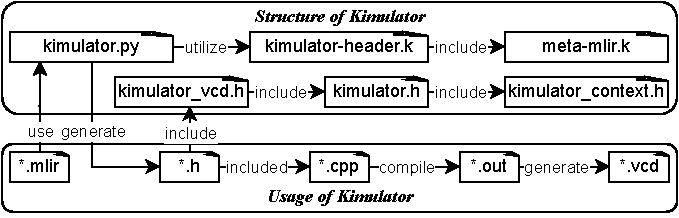
\includegraphics{fig/k-circt-kimulator-structure.drawio.pdf}
    \caption{The structure of kimulator.}
    \label{fig:kimulator-structure}
\end{figure}

\smallskip
\textbf{Usage of Kimulator}.
From the usage perspective, \textit{kimulatot.py} and \textit{kimulator\_vcd.h} are two key components in kimulator. \textit{kimulatot.py} is used to parse the CIRCT source file and generate headers to leverage the CIRCT formal semantics in $\mathbb{K}$. \textit{kimulator\_vcd.h} is included in these headers, providing functions for the hardware module manipulation and semantics activation. Using these functions, users then can develop a Cpp file for simulation. In the file, users can stimulate hardware modules several times. After compiling the developed source file, users can analyze the simulation results from the generated VCD file. Without our interface, users must have a strong familiarity with the $\mathbb{K}$ framework, as well as view and modify the result in the complex Kore language. In other words, we provide a simple way to use the formal semantics, shielding the complexity of formality and $\mathbb{K}$.

Compared to the famous open-source simulator \textit{verilator}, our work does not introduce more labor to simulation due to the usage of a formal framework. \red{For example, Fig.~\ref{fig:kimulator-example} provide crafted C++ source files for Fig.~\ref{fig:circt-example} in both kimulator and verilator. Explain verilator source file. Compare to kimulator source file. Thus, reducing the learning cost of using our framework.}

\begin{figure}[th]
    \centering
    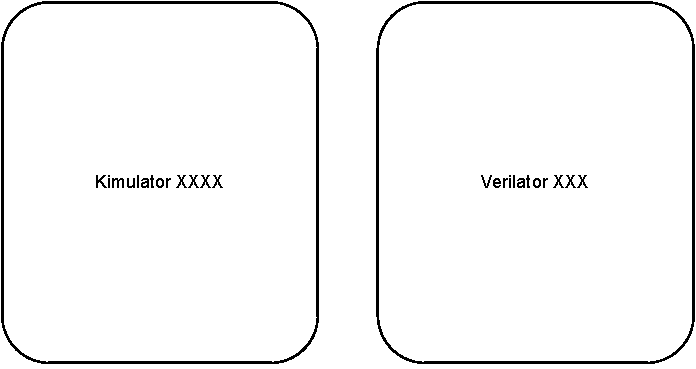
\includegraphics{fig/k-circt-simulation-example.drawio.pdf}
    \caption{\red{A simple simulation example for kimulator and verilator.}}
    \label{fig:kimulator-example}
\end{figure}

\smallskip
\textbf{Structure of Kimulator}. From the key components (i.e., \textit{kimulator.py} and \textit{kimulator\_vcd.h}), we delve into the details of kimulator. \textit{kimulator.py} is a script that employs \textit{krun} to use the \textit{kompile}d \textit{kimulator-header.k} and extracts headers from the result, where \textit{krun} and \textit{kompile} are $\mathbb{K}$ provided tools for interpretation and generation of the tools like \textit{krun}, respectively. Inside of \textit{kimulator-header.k}, we leverage the phases provided by MLIR static semantics in \textit{meta-mlir.k} to generate Cpp representation for its corresponding CIRCT hardware module. This representation is an instance of the class \textit{KimulatorModel} in \textit{kimulator.h}, which provides functions to set variables in modules and evaluate the results according to the module input. The evaluation is completed by \textit{krun}ing the core dialect semantics. We make the execution process continuous (i.e., pick up the previous state to continue execution after modifying the simulation time) by working on Kore language, which is an intermediate language that \textit{krun} can continue its execution on. The representation's variables also update after evaluation by extracting the information in the Kore language. \textit{kimulator-context.h} provides class \textit{KimulatorContext} to hold global information for evaluation (e.g., simulation time), while \textit{kimulator\_vcd.h} offers the ability to store the simulation results in VCD file.

In conclusion, kimulator provides a user-friendly interface similar to verilator for simulation using our CIRCT formal semantics, while avoiding complex concepts in formal method and $\mathbb{K}$ framework.